\section{Introduction}
\label{sec:introduction}

\subsection{isMOOD: Main Attributes \& Activities}
\label{subsec:ismood}

During the final semester of my studies
at the Athens University of Economics and Business, Greece,
from March--June 2019,
I implemented my internship
at isMOOD Data Technology Services.\footnote{\url {https://www.ismood.com}}

isMOOD is a company in the field of social media analytics.
The company collects data from social networks
and transforms them to useful knowledge for companies.
Their vision is to transform social media analytics
into an actionable decision making tool.
Therefore, the company has developed an in-house web platform,
through which a company-client is informed
on what people say about them, their products and competitors,
captures their customers' sentiment and needs,
and ultimately understands their audience.

The particular platform is a proactive and strategic tool for prediction
due to the fact that historical data are maintained.
By studying and analyzing them,
a company can address potential threats
and take actions to avoid them.
As a result, better brand management may be achieved,
along with better crisis management and scenario analysis.

Another asset of the platform is the identification
of a company's influencers.
By identifying their influencers,
a company has the opportunity
to convert them into advocates,
by sharing positive content about their brand, campaign or product.
At the same time, the company can facilitate 
from isMOOD's World of Mouth techniques,
in order to enhance their virality,
interact with their market,
and raise their audience's positive engagement.

Apart from the platform,
isMOOD also offers customised reports to companies-clients.
These reports include information on a company's impact
at social media in a particular time range,
along with sentiment progress.
The reports contain certain insights
derived from isMOOD's platform,
such as top comments and average sentiment,
but in addition,
they offer business insights and suggestions
derived from the isMOOD personnel itself.

\subsection{isMOOD: Organisation Structure}
\label{subsec:ismood-structure}

isMOOD consists of two main teams;
the Business team and the Technical team.
The Business team is responsible
for the abovementioned reports,
the assistance and communication with the clients,
the arrangement of the offers that are provided to them,
and the insurance of their overall contentment.
On the other hand, the Technical team is responsible
for the development, maintenance and security
of the isMOOD platform,
along with everything related to the company's digital activities.

isMOOD aims to bridge the gap between technology and people,
thus both teams are equally critical
for the company's smooth operation.
The two teams are in constant communication with each other,
and with the Project Manager,
a person also responsible
for the operation of the logistics and financing activities.
All the personnel is supervised by the Managing Director,
who also operates the company's sales and marketing activities.

The company's organisation structure as described above
is illustrated in the following figure.

\begin{figure}[ht]
\centering
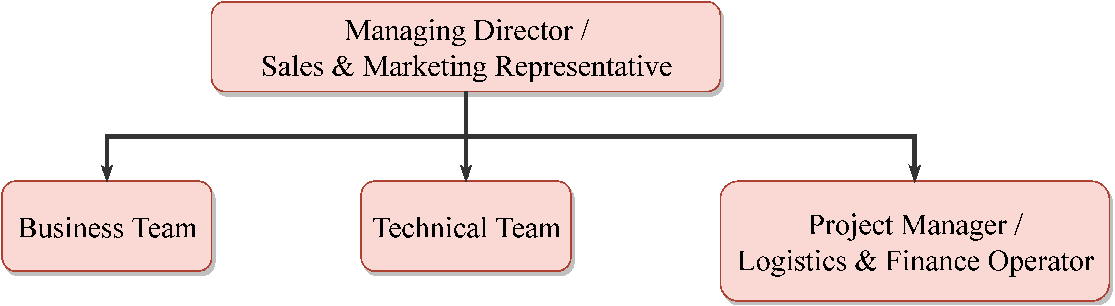
\includegraphics[width=\textwidth]{ismood-org-chart.eps}
\caption{isMOOD Organisation Chart}
\label{fig:ismood-org-chart}
\end{figure}

\subsection{Internship Goals}
\label{subsec:internship-goals}

Through my insternship at isMOOD company
I aimed to accomplish a variety of goals.
First of all, I wanted to advance my technical skills.
Particularly, I attempted to increase my experience with Python.
It was also my intention to get more familiar with NoSQL databases,
and isMOOD could provide that to me
since they use MongoDB and Elasticsearch.

During my internship I was assigned a particular project
that involved a lot of research.
This project was related to Text Analytics,
specifically Sentiment Analysis,
research areas I am interested in.
Thus, through studying a variety of published research work,
I attempted to familiarise with the abovementioned areas.

Apart from technical knowledge,
this internship formed my first work experience.
I was finally in a real work environment,
working for actual clients
under real working conditions
in fixed work shifts,
being in constant collaboration with other employees
and supervised for my progress.
Despite having worked on multiple group projects
at University before,
it was this internship that would teach me
the actual impact of a project
and the consequences of failures and inconsistencies;
working for actual clients instead of a course grade
provides a completely different perspective on a project.

\subsection{Final Report Goals}
\label{subsec:report-goals}

Through the implementation of my final report,
I attempt to evaluate the knowledge, experience,
and overall impact of my internship.
This report provides a thorough description
of my three-month activities and evolution at isMOOD,
my final thoughts on the company,
my colleagues and supervisors,
the project I worked on, and
the benefits I earned.
